\index{Excel data}
\index{Parameter!Excel file}
In the \gdpropview{}, you can add Excel files to \gdcases{} which contain parameters referenced from the \gdcases{} or \gdsteps{} they contain. 
\begin{enumerate}
\item Navigate to the \gdpropview{} for the \gdcase{} you want to add the Excel file to. 
\item Enter the path to the Excel file in the \bxname{Excel data file} field. 

The path to the Excel file can be absolute or relative (if you have specified a data files path \bxpref{gdprefs}).

\bxtipp{The Excel file must be configured in a specific way in order for \jb{} to read it \bxpref{TasksConfigureExcel}}.

\item If you reuse this \gdcase{}, the Excel file you enter will be reused along with the \gdcase{}. When you reuse the \gdcase{}, you can choose whether you leave this file or change it for another one. 
\bxtipp{If you store your Excel files in your workspace, you will be able to open these directly in \jb{} from the navigator view using the in-place editor. }
\item A \gdcase{} you have added an Excel file to is marked with a small Excel icon in the browsers to help you find it more easily later. 
\bxwarn{Please note that the Excel file is read at the start of the test execution. Any changes to the file after this will not affect the test data. For information on using the date function in Excel, see the section later \bxpref{exceltoday}.}
\end{enumerate}

\subsubsection{Configuring the Excel file}
\index{Excel File Configuration}
\label{TasksConfigureExcel}
\begin{itemize}
\item The worksheet in Excel must be named with the language code for the language your data are in. See the Reference Manual (\bxextref{\jb{}efman}{ref,langcodes}) for a list of language codes.

For example, if the data of your first sheet are for French, then name the first sheet: \bxshell{fr\_FR} (\bxfigref{excel}).

\begin{figure}[h]
\begin{center}
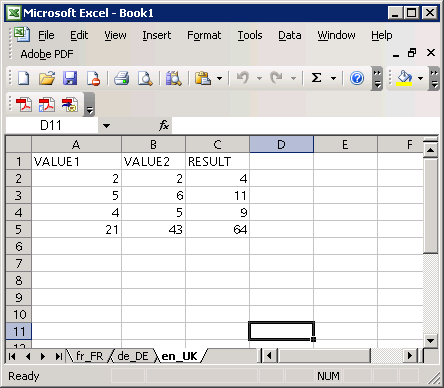
\includegraphics{Tasks/Testdata/PS/excelexample}
\caption{Example Excel Table}
\label{excel}
\end{center}
\end{figure}

You can create sheets for every language you need. Make sure that each sheet is named with the language code. 
\jb{} will read the sheet which corresponds to the working language when the test is being executed. 

\item Name the top cell of each column with a parameter name from your \gdcase{}.

For example, if you entered the reference \bxcaption{=VALUE1}, then you must enter \bxshell{VALUE1} in the top cell of the column which will contain data for that parameter. 
\bxtipp{\jb{} is case sensitive.}
\item Make sure that all the parameters for your \gdcase{} have a column.
\item Do not leave any gaps in the table.
\item You must have an entry for each parameter used in the \gdcase{}. 
\item You can then fill in the values or formulae you want to use for these parameters. Each row in the table represents one set of data for the parameters used. 
\bxtipp{We recommend that you format cells as text \emph{before} adding the test data. This ensures that Excel's number formatting won't modify the test data in unexpected and undesirable ways. Especially for the boolean values\bxname{true} and \bxname{false}, make sure you format the column as text.}
\item If your Excel table contains data which change from day-to-day, then make sure you open the file before starting your test. Otherwise, the data from the last-opened state will be used.
\bxtipp{If you store your Excel files in your workspace, you will be able to open these directly in \jb{} from the navigator view using the in-place editor. }
\item See the section later on using the \bxname{today} function in Excel to get the current date \bxpref{exceltoday}. 
\item Excel files may not contain autofilters in any of the worksheets to be used as data sources for \jb{}. Remove any filters from all your Excel sheets before running a test. 
\end{itemize}

\subsubsection{Using the =TODAY() function in Excel}
\index{Excel TODAY function}
\label{exceltoday}
\begin{enumerate}
\item Because Excel stores the \bxcaption{=today()} function as a six-digit number, you must use a particular process to use this function to check a date as part of a test.
\item Enter the function \bxshell{=today()} in a a different sheet to the one you are using for your data sets. You can enter it in the same sheet if you want to, but make sure that it has its own column. It must not be in one of the columns you will use as a data set.
\item For example, your =today() function is in sheet one, cell G4.
\item You want your date to appear as dd.mm.yyyy.
\item In the column for your data set, enter the following formula:
\begin{quote}
=text(Sheet1!G4, ''dd.mm.yyyy'')
\end{quote}
\item This will mean that the date will be treated as it appears with Excel. 
\bxtipp{If you are using the =today() function, don't forget to open the Excel file before  starting your test. Otherwise, the data from the last-opened state will be used.}
\bxtipp{If you store your Excel files in your workspace, you will be able to open these directly in \jb{} from the navigator view using the in-place editor. }
\end{enumerate}

